
The content in this document is taken verbatim from \cite{Willers2013}.

\index{case study!laser rangefinder range equation|(}\index{laser rangefinder!range equation case study|(}

\noindent
In this section the range equation for a laser rangefinder is derived. Because the radiometry techniques developed in this book do not cover coherent sources, an explanation is in order. In this rangefinder application  the laser is used as a source with very high radiance. Laser rangefinders operate on the principle that light travels approximately 300~mm distance in one nanosecond. The time elapsed between the transmission of the pulse and the reception of the pulse is used to determine the distance. This specific analysis does not require the laser to be considered as a coherent source, and hence the radiometry techniques in this book can be used here. These techniques cannot be readily used for problems concerned with spatial or temporal coherence.

In most laser rangefinders the transmitter and receiver are co-located and co-axial on the same optical path. If a laser pulse
is directed to an object and reflected back from the object, the elapsed time between the departure and arrival of the reflected light pulse is an indication of the distance to the object. The objective with this analysis is to derive an expression for the SNR for the laser rangefinder. The  SNR can then be used to investigate the effect of several design parameters on system performance. For another approach to the range equation for laser rangefinders, see Kaminsky.\cite{Kaminski1980}



\subsection{Noise equivalent irradiance\index{laser rangefinder!noise equivalent irradiance (NEE)}\index{irradiance!noise equivalent (NEE)|seealso{laser rangefinder example}}}
\noindent
The noise equivalent irradiance in the receiver is given by \cite{Willers2013}
\begin{eqnarray}
NEE&=& \frac{
\sqrt{\Delta f A_d}
}{
D^\ast A_1 \tau_a
},
\label{lrfnoise}\label{laserrxn}
\end{eqnarray}
where 
$A_d$ is the detector area, 
$\Delta f$ is the noise bandwidth in the receiver, 
$A_1$ is the receiver aperture area, and 
$\tau_a$ is the receiver filter transmittance. The
$D^\ast$ values can include all of the relevant noise terms such as detector noise, amplifier noise, background induced noise, and system noise. 
For the purposes of this chapter, we will only work with a single $D^\ast$, assuming that all noise sources are incorporated in this value.
The method whereby these noises are all combined into a single $D^\ast$ follows from noise power addition. If the different noise sources are uncorrelated, originating from different components each with individual, statistically independent processes, it can be shown that \textit{for uncorrelated sources},  noise \textit{power} adds linearly. The total noise is then given by
\begin{equation}
i_{\rm eff}=\sqrt{\sum_0^N i_n^2}\;\;,\label{eq:combinenoisesources}
\end{equation}
where there are $N$ noise sources $i_n$. The individual noise sources in this equation can be either spectral noise [A$\sqrt{\rm Hz}$] or integrated wideband noise [A].

A little care must be taken with noise expressed in terms of $D^\ast$. In this case $D^\ast$ corresponds to the signal itself, not the noise it `mimics.' 
Like noise $D^\ast$ also adds in quadrature,
\begin{equation}
\frac{1}{D^\ast_{\rm eff}}=\sqrt{\sum_0^N 
\frac{1}{\left(D^\ast_n\right)^2}
}\;.\label{eq:combinenoiseDeeStar}
\end{equation}
\index{power spectral density (PSD)!combining spectra|)}


\begin{figure}[t]
\centering
\resizebox{0.8\textwidth}{!}{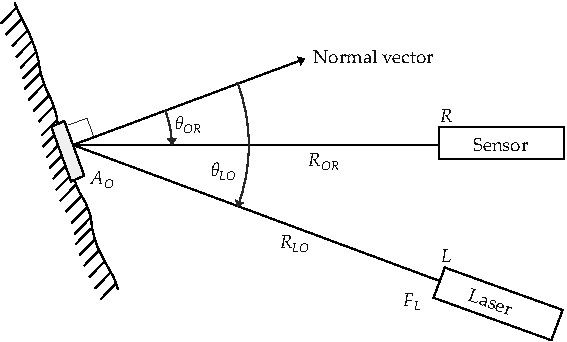
\includegraphics{pic/rangelay.pdf}}
\caption{Laser rangefinder layout.
\label{rangelay}}
\end{figure}


\subsection{Signal irradiance\index{laser rangefinder!signal irradiance}}
\noindent
The geometrical relationship between the laser transmitter, the object, and the laser receiver is shown in Figure~\ref{rangelay}. The laser power or flux is denoted by $\Phi_L$ (in watts), the distance from the laser to the object is $R_{LO}$, and the distance from the object to the receiver is $R_{OR}$. The illuminated object-surface normal vector makes an angle $\theta_{LO}$ with the laser illumination direction, and an angle $\theta_{OR}$ with the receiver sightline direction.

Several simplifying assumptions are made in order to simplify the problem and emphasize the methodology. The receiver and transmitter fields are co-axial, and the receiver and transmitter are located at the same position. Hence, the distance from the object to the laser transmitter is equal to the distance from the object to the laser receiver, and the same atmospheric transmittance applies to both optical paths.

From the definition of radiance \cite{Willers2013} radiance values at both surfaces are
\begin{equation}
L_{01}=\frac{\cjwmypartial^2 \Phi}{\cjwmypartial{}A_0\,\cos\theta_0\,\cjwmypartial\Omega_1}\label{cc1}
\end{equation}

The laser beam radiance is calculated from the definition of radiance in \myeqno{cc1}, requiring the optical power, beam area at the source and beam solid angle (divergence).  In order to use this very simple equation, the Gaussian shape properties of the laser beam is discarded for two very simple uniform shapes.
The laser beam angular radiance distribution is assumed to be uniform within the top-hat-shaped beam divergence profile (e.g., peak normalized divergence). The laser beam power distribution is assumed to be uniform across the area of the beam (e.g., peak normalized area). Using \myeqno{cc1} and these two simplifications, the radiance can be written as
\begin{equation}
L_L=\frac{\Phi_L}{\Omega_L A_L},\label{fig:laserrangeirrad}
\end{equation}
where $\Omega_L$ is the laser beam solid angle, and $A_L$ is the laser beam cross-section area at the laser source. This simplification might not satisfy the required mathematical gaussian beam rigor, but it does provide order-of-magnitude radiance estimates.

\textit{\index{irradiance!radiant}Irradiance} is derived as (note the $\cos\theta_1$ term)
\begin{equation}
E=\frac{\cjwmypartial{}\Phi}{\cjwmypartial{}A_1\,}=
\frac{L\,\cjwmypartial{}A_0\,\cos\theta_0\cos\theta_1}{R_{01}^2}=L\,\Omega_0\,\cos\theta_1.
\label{irradef}
\end{equation}
From \myeqnos{irradef}{fig:laserrangeirrad}, the irradiance on the object is then 
\begin{eqnarray}
E_O&=&\frac{L_L A_L \tau_{OL}\;\cos\theta_L\cos\theta_{LO}}{R^2_{LO}}\nonumber\\
&=&\frac{\Phi_L \tau_{OL}\cos\theta_{LO}}{\Omega_L R^2_{LO}},
\end{eqnarray}
where it is assumed that $\cos\theta_{L}=1$ because the laser beam radiates perpendicularly from the laser mirror. The uncooperative target object can have any orientation relative to the laser beam, denoted by $\theta_{LO}$.


\subsection{Lambertian target reflectance\index{laser rangefinder!Lambertian reflective surface|(}}
\noindent
The laser pulse falling onto the object is reflected by the object. Most
natural surfaces have diffuse reflectance and scatter energy in all
directions (a Lambertian surface). The reflected laser spot on the target object has a radiance of
\begin{equation}
L_O=\frac{\rho E_O}{\pi}=\frac{\rho\Phi_L \tau_{LO}\cos\theta_{LO}}{\Omega_L
\pi R^2_{LO}}.\label{loo}
\end{equation}


%============================================================

The irradiance, caused by the reflected pulse, at the laser receiver is then, from \myeqno{irradef},
\begin{eqnarray}
E_R&=&\frac{\Phi_R}{\cjwmypartial A_1}\nonumber \\
&=&\frac{L_O A_O \cos\theta_{OR}\tau_{OR}}{R_{OR}^2},
\end{eqnarray}
where $A_O$ is the area illuminated by the laser that is visible to the
sensor. Further manipulation using \myeqno{loo} leads to
\begin{eqnarray}
E_R&=&\frac{\Phi_L \tau_{LO}\cos\theta_{LO}\rho A_O \cos\theta_{OR}\tau_{OR}}
{\Omega_L \pi R^2_{OR}R^2_{LO}}\nonumber \\
&=&\frac{
\rho \Phi_L \tau_{LO} \cos\theta_{LO} A_O \cos\theta_{OR} \tau_{OR}
}{
\pi \Omega_L R^2_{LO}R^2_{OR}
}.
\end{eqnarray}
By co-locating the laser transmitter and the receiver ($R^2_{LO}=R^2_{OR}=R$, $\tau_{LO}=\tau_{OR}=\tau_a$, and $\cos\theta_{LO}= \cos\theta_{OR}$) the expression for irradiance simplifies to
\begin{equation}
E_R = \frac{
(\rho \cos^2\theta_{LO} A_O)
\Phi_L \tau^2_{a}
}{
\pi \Omega_L R^4
},\label{radar}
\end{equation}
where $R$ is the distance between the object and the rangefinder.
\myeqno{radar} is similar to the radar range equation. The product $\rho\cos^2\theta_{LO} A_O$ can be regarded as the \index{laser rangefinder!target optical cross section}target optical cross-section. In the radar case, the optical cross section has a fixed magnitude irrespective of distance between the laser and target object. This is also true for a laser rangefinder illuminating an airborne object where there is no reflective background.  If the object is observed against a terrain background, the terrain background also contributes to the reflected signal (depending on the geometry).


%++++++++++++++++++++++++++++++++++++++++++++++++++

\subsection{Lambertian targets against the sky}

\noindent
The rangefinder irradiance SNR is the ratio of signal strength
[\myeqno{radar}] to noise [\myeqno{lrfnoise}], and is given by
\begin{eqnarray}
\frac{E_R}{NEE}&=&\frac{
\frac{
\rho \Phi_L \tau^2_{a} \cos^2\theta_{LO} A_O
}{
\pi \Omega_L R^4 }
}{\frac{\sqrt{\Delta f A_d}}{D^\ast A_1 \tau_a}}\\
&=&\frac{\rho\Phi_L
\tau_{a}^2 \cos^2\theta_{OR}A_0D^\ast A_1 \tau_a} { \pi\Omega_L R^4
\sqrt{\Delta f A_d}}.
\end{eqnarray}

If Bouger's law is accepted for atmospheric transmittance, the transmittance can be written in terms of distance as $\tau_a=e^{-\gamma R}$. The laser flux is given by $\Phi_L\approx Q_L/t_p$, where $Q_L$ is the pulse
energy in [J], and $t_p$ is the pulse width in [s]. The required receiver
electronic noise bandwidth can be written in terms of the pulse width as
$\Delta f=k_nk_f/t_p$, where 
$k_n$ relates the electrical system electronic bandwidth with the noise equivalent bandwidth, and 
$k_f$ relates the laser pulse width with the system electronic bandwidth (see \cite{Willers2013} for both definitions).

The irradiance SNR can now be written as
\begin{equation}
\frac{E_R}{NEE}=
\overbrace{
\left(\frac{A_0\rho \cos^2\theta D^\ast }{\pi \sqrt{k_nk_f}}\right)
}^{\rm no\;\;control}
\overbrace{
\left(\frac{Q_L A_1 \tau_a }{\Omega_L\sqrt{t_p A_d}}\right)
}^{\rm design}
\overbrace{
\left(\frac{e^{-2\gamma R} }{R^4}\right).\\
}^{\rm distance}
\label{lrfd2}
\end{equation}
In \myeqno{lrfd2} there are three groups of variables:

\begin{enumerate}[1.]

\item 
Variables and constants that the designer has no control over, such as the object orientation and reflectivity, $D^\ast$, and constants.

\item 
Variables that the designer controls in the design process, such as laser energy, receiver aperture area, laser pulse width, and detector size.

\item 
Distance-related factors that the designer has little control over.

\end{enumerate}

The designer can now easily determine that increased laser energy and receiver aperture improves the SNR linearly, whereas increased detector area and pulse width decrease the SNR. Contrary to intuition, a longer pulse width (i.e., a lower electronic bandwidth) decreases the SNR. Why?

%++++++++++++++++++++++++++++++++++++++++++++++++++

\subsection{Lambertian targets against terrain}
\noindent
If the laser rangefinder is viewing targets against the terrain, the laser light is reflected from the target object as well as its  surrounding terrain. This implies that the real target area is not of sole importance because the terrain background also reflects the laser pulse. There are two possibilities regarding the laser transmitter and receiver beam or FOV sizes.

Note that $\frac{E_R}{NEE}=SNR$, which is the signal-to-noise ratio.

If the receiver FOV  is larger than the transmitter beam width, the receiver sees the whole laser spot. This implies that the effective laser spot area is defined by the laser beam width by
\begin{equation}
\Omega_L=\frac{A_O\cos\theta_{LO}}{R^2},
\end{equation}
and hence \myeqno{radar} --- the irradiance at the receiver ---  becomes
\begin{equation}
E_R = \frac{
\rho \Phi_L \tau^2_{a} \cos\theta_{LO}}{\pi R^2 }\label{lrfi1}, 
\end{equation}
hence, and assuming that the target and background has the same reflectance across the laser spot:
\begin{equation}
SNR=
\overbrace{
\left(\frac{\rho \cos^2\theta D^\ast }{\pi \sqrt{k_nk_f}}\right)
}^{\rm no\;\;control}
\overbrace{
\left(\frac{Q_L A_1 \tau_a }{\sqrt{t_p A_d}}\right)
}^{\rm design}
\overbrace{
\left(\frac{e^{-2\gamma R} }{R^2}\right).\\
}^{\rm distance}
\label{lrfd2d}
\end{equation}


If the receiver FOV is smaller than the transmitter beam width, the receiver only views a portion ($A_O^\prime<A_O$) of the whole laser spot. This implies that the effective laser spot area is determined by the receiver FOV footprint  $A_O^\prime$ as 
\begin{equation}
\Omega_R=\frac{A_O^\prime\cos\theta_{LO}}{R^2},
\label{eq:lrfFOVsmaller}
\end{equation}
and hence \myeqno{radar} becomes
\begin{equation}
E_R = \frac{
\rho \Phi_L \tau^2_{a} \cos\theta_{LO}}{\pi R^2 }\Upsilon , %\frac{\Omega_R}{\Omega_L}
\label{lrfi2}
\end{equation}
where $\Upsilon =\Omega_R/\Omega_L$ is the fraction of the laser spot
viewed by the laser receiver FOV, and $0\leq\Upsilon\leq 1$. 
hence, and assuming that the target and background has the same reflectance across the laser spot:
\begin{equation}
SNR=
\overbrace{
\left(\frac{\rho \cos^2\theta D^\ast }{\pi \sqrt{k_nk_f}}\right)
}^{\rm no\;\;control}
\overbrace{
\left(\frac{Q_L A_1 \tau_a \Upsilon}{\sqrt{t_p A_d}}\right)
}^{\rm design}
\overbrace{
\left(\frac{e^{-2\gamma R} }{R^2}\right).\\
}^{\rm distance}
\label{lrfd2e}
\end{equation}
When comparing
\myeqnos{lrfi1}{lrfi2}, we see that they are the same, except
for the fraction $\Upsilon$. \myeqno{lrfi2} is the more general case
because \myeqno{lrfi1} is a special case when $\Upsilon=1$.
\index{laser rangefinder!Lambertian reflective surface|)}



\subsection{Quadrant detectors}
\noindent
Laser guided sensors all employ quadrant detectors.  The detector shape is normally round, divided into four equal-sized, radial sector-shaped quadrants, each of these quadrants in effect is a separate detector. Suppose that in the initial detection phase of acquisition, the laser flux may fall only on a single quadrant.  After initial acquisition, when tracking the target, the (defocused) laser flux is spread approximately equal between the four quadrants.

Hence, when considering the requirement to track the spot, the beam flux must be divided by four to obtain the signal strength on one quadrant of the detector. The SNR is then given by

\begin{equation}
SNR_Q=
\overbrace{
\left(\frac{\rho \cos^2\theta D^\ast }{\pi \sqrt{k_nk_f}}\right)
}^{\rm no\;\;control}
\overbrace{
\left(\frac{(Q_L/4) A_1 \tau_a \Upsilon}{\sqrt{t_p A_d/4}}\right)
}^{\rm design}
\overbrace{
\left(\frac{e^{-2\gamma R} }{R^2}\right).\\
}^{\rm distance}
\label{lrfd2f}
\end{equation}
where the signal is divided by four when tracking perfectly and the area of the detector also divides by four.


The general form that models both detection and tracking would be
\begin{equation}
SNR_Q=
\overbrace{
\left(\frac{\rho \cos^2\theta D^\ast }{\pi \sqrt{T k_nk_f}}\right)
}^{\rm no\;\;control}
\overbrace{
\left(\frac{Q_L A_1 \tau_a \Upsilon}{\sqrt{t_p A_d}}\right)
}^{\rm design}
\overbrace{
\left(\frac{e^{-2\gamma R} }{R^2}\right).\\
}^{\rm distance}
\label{lrfd2g}
\end{equation}
where $T=1$ for detection and $T=4$ for tracking.




\subsection{Detection range\index{laser rangefinder!detection range}\index{detection!range}}
\noindent
The equations in the previous section provide the signal strength obtained from a laser transmitter at a laser receiver. An estimate of the detection range can be obtained by solving the range equation
\begin{equation}
SNR=\frac{E_R(R)}{NEE},
\label{eq:laserdetectionsnrerror}
\end{equation}
where $SNR$ is the signal-to-noise ratio required to achieve detection. Solving the detection range problem means finding a value for range $R$ in \myeqno{lrfd2} that would yield the required SNR. 


\subsection{Example calculation\index{laser rangefinder!example calculation!range equation|(}\index{detection!range example calculation|(}}
\noindent
\myeqno{lrfd2} is known as the laser rangefinder range equation because the range may be solved for a given set of design choices and SNR. One such solution is shown here.  The values shown in Table~\ref{tab:rangefinderparameters} were used in the calculation.



\begin{table}[tb]
\centering
\caption{Parameters used in rangefinder example. \label{tab:rangefinderparameters}}
{\small
\begin{tabular}{%
%|c|c|c|%
%|c|c|c|%
|C{17mm}|C{16mm}|C{19mm}|%
C{17mm}|C{16mm}|C{16mm}|%
}
\hline
\textbf{Para\-meter} & \textbf{Value} & \textbf{Units}& \textbf{Para\-meter} & \textbf{Value} & \textbf{Units}\\
\hline
$\tau_a$&0.5 & & $\rho$&0.1& \\
$A_1$ & $2\times10^{-3}$ &m$^2$ & $\cos\theta$ & 0.5 &  \\
$k_n$ & 1 & & $\Upsilon$ & 1 &\\
$k_f$ & 1 & & $\lambda$&1.06& \si{\micro\metre}{}\\\
$\Omega$ & $1\times10^{-3}$ &sr & $Q_L$ & 0.06 & J \\
$f/\#$ & 1.4 & & $\Phi$ & 4 & MW\\
$f$ & 0.07& m & $t_p$ & 15 & ns\\
$D^\ast$ & $3\times10^{11}$& cm$\cdot$$\sqrt{\rm Hz}$W$^{-1}$ &$\cjwmypartial \lambda$& 0.02&\si{\micro\metre}{}  \\
$A_d$ & $4.6\times10^{-6}$& m$^2$ &&&\\
\hline
\end{tabular}
}
\end{table}

\myeqno{lrfd2} was used to calculate the SNR versus range for several atmospheric conditions. The atmospheric attenuation coefficients used here\cite{EOHandbook1974} were $\gamma = 0.17$, $0.33$, $0.53$, and $0.88$, corresponding to meteorological ranges of 15~km, 8~km, 5~km, and 3~km at the laser wavelength of 1.06~\si{\micro\metre}{}.   A graph indicating SNR versus range is shown in Figure~\ref{kamif}. Note how strongly the atmospheric attenuation influences the range performance of the rangefinder. Figure~\ref{kamif} also shows the expected operational range as a function of detector $D^\ast$. 

The \index{detector!signal voltage}\index{signal!voltage}signal voltage, for a target with uniform surface radiance, is \cite{Willers2013} 
\begin{equation}
\cjwmypartial v_{\cal S}=
\frac{k \,\widehat{{\cal R}}\, Z_t \,dA_{0}\,\cos\theta_0\,
\,A_{1} 
}{R_{01}^2}
\int_{0}^{\infty}
 \epsilon_{0\lambda} L_{0\lambda}
\,\tau_{a\lambda} {\cal S}_\lambda
\cjwmypartial\lambda,
\label{eq:sensoroutputvoltage}
\end{equation}
where
$v_{\cal S}$ is the detector voltage [V] for flux in the band defined by ${\cal S}$, for elemental source area $dA_{0}$.  \myeqno{eq:sensoroutputvoltage} can be integrated over the source area to obtain the full source signature:
\begin{equation}
 v_{\cal S}=
 k \,\widehat{{\cal R}}\, Z_t\,A_{1} 
\int_{A_0} \left(
\frac{1}{R_{01}^2}
\int_{0}^{\infty}
 \epsilon_{0\lambda} L_{0\lambda}
\,\tau_{a\lambda} {\cal S}_\lambda
\cjwmypartial\lambda\right) dA_{0}\,\cos\theta_0
.
\label{eq:sensoroutputvoltage1}
\end{equation}


The background flux in the scene determines the detector current, which in turn determines  the noise in the detector. If the sensor is operating at night, the detector noise is at a minimum. If the sensor is pointed at a bright, sunlit background, the current and hence the noise in the detector increases relative to the dark night condition.  By converting the background flux noise to $D^\ast$, the range versus $D^\ast$ graph can be used to predict degradation in system performance under bright sunlight conditions.  Typical background radiance values are shown in Table~\ref{tab:rangefinderperformance}. The background radiance values were used to calculate the current in the detector using a variation of \myeqno{eq:sensoroutputvoltage}.  Once the current in the detectors were known, the shot noise at the respective currents were calculated, and finally, new $D^\ast$ values were calculated using \myeqno{eq:combinenoiseDeeStar}.  These new $D^\ast$ values now represent the noise performance of the sensor under the various background conditions. Once the new $D^\ast$ values were known, the range performance corresponding to the different conditions were determined from the bottom graph in Figure~\ref{kamif}.  The operating ranges are also shown in Table~\ref{tab:rangefinderperformance}.


\begin{table}[tb]
\centering
\caption{Background radiance at 1.06 \si{\micro\metre}{}, expressed as a detector $D^\ast$ and resultant operating range \cite{Kaminski1980}.\label{tab:rangefinderperformance}}
\begin{tabular}{|l|c|c|c|c|}
\hline
\textbf{Terrain} & \textbf{Background} & \textbf{Background} & \textbf{Effective} & \textbf{Range} \\
         & \textbf{Radiance} &$\bm{D^\ast}$&$\bm{D^\ast}$ & \\
\hline
Dark night   & 0    & $\infty$               & $3\times10^{11}$ &6.64 \\
Grass terrain & 10 & $6\times10^{11}$ &$2.7\times10^{11}$ & 6.32\\
Snow terrain & 100 &$2\times10^{11}$ &$1.67\times10^{11}$ &5.79 \\
\hline
Blue sky & 10 &$6\times10^{11}$ &$2.7\times10^{11}$ & 6.32\\
Dark clouds & 8 &$7\times10^{11}$ &$2.75\times10^{11}$  &6.34 \\
Sunlit clouds & 100 & $1.7\times10^{11}$ &$1.48\times10^{11}$ &5.62 \\
\hline
& W/(m$^2$$\cdot$sr$\cdot$\si{\micro\metre}{}) & cm$\cdot$$\sqrt{\rm Hz}$/W & cm$\cdot$$\sqrt{\rm Hz}$/W  & km\colheightrule\\
\hline
\end{tabular}
\end{table}

% two plots
\begin{figure}[tb]
\centering
\resizebox{115mm}{!}{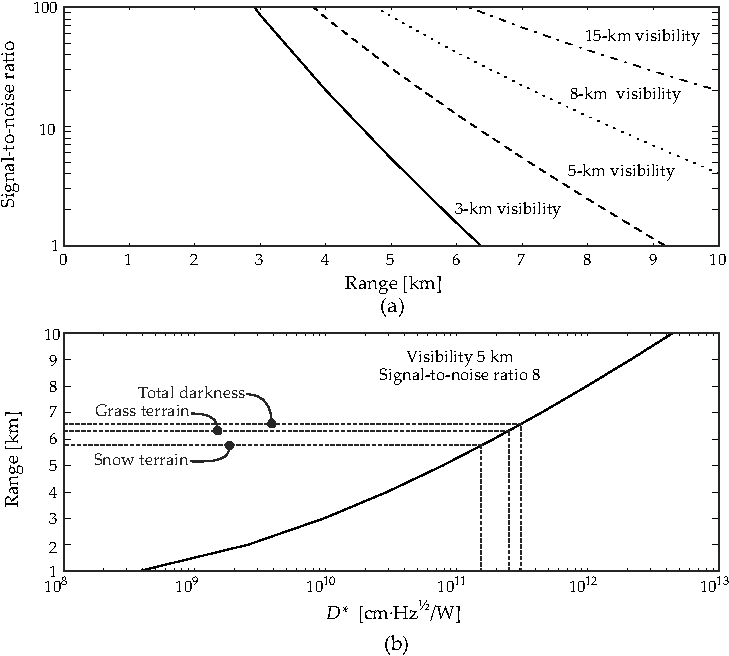
\includegraphics{pic/eosdrf.pdf}}
\caption
{\label{kamif}Laser-rangefinder range equation analysis: (a)~SNR versus range for several atmospheric visibility values and (b)~expected range as a function of detector $D^\ast$.}
\end{figure}

\index{detection!range example calculation|)}
\index{laser rangefinder!example calculation!range equation|)}

\begin{figure}[t]
\centering
\resizebox{5in}{!}{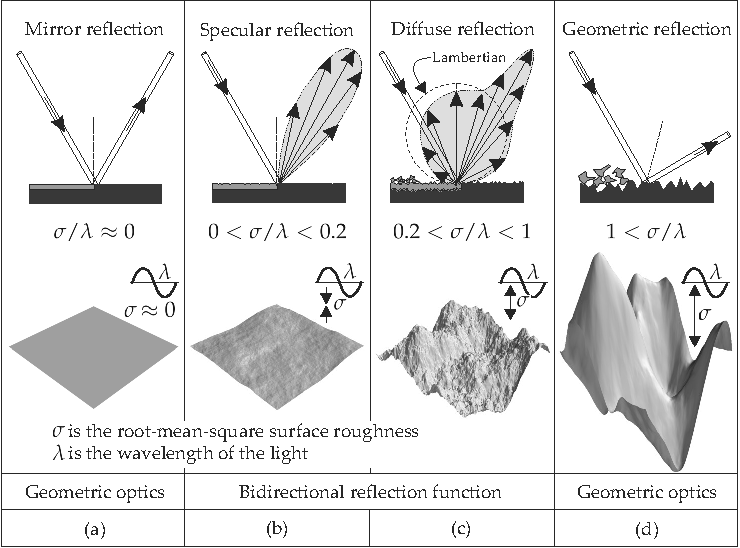
\includegraphics{pic/nonlambert.pdf}}
\caption{Micro-scale surface roughness and reflection.\label{nonlambert}}
\end{figure}

\begin{figure}[bt]
\centerline{\resizebox{125mm}{!}{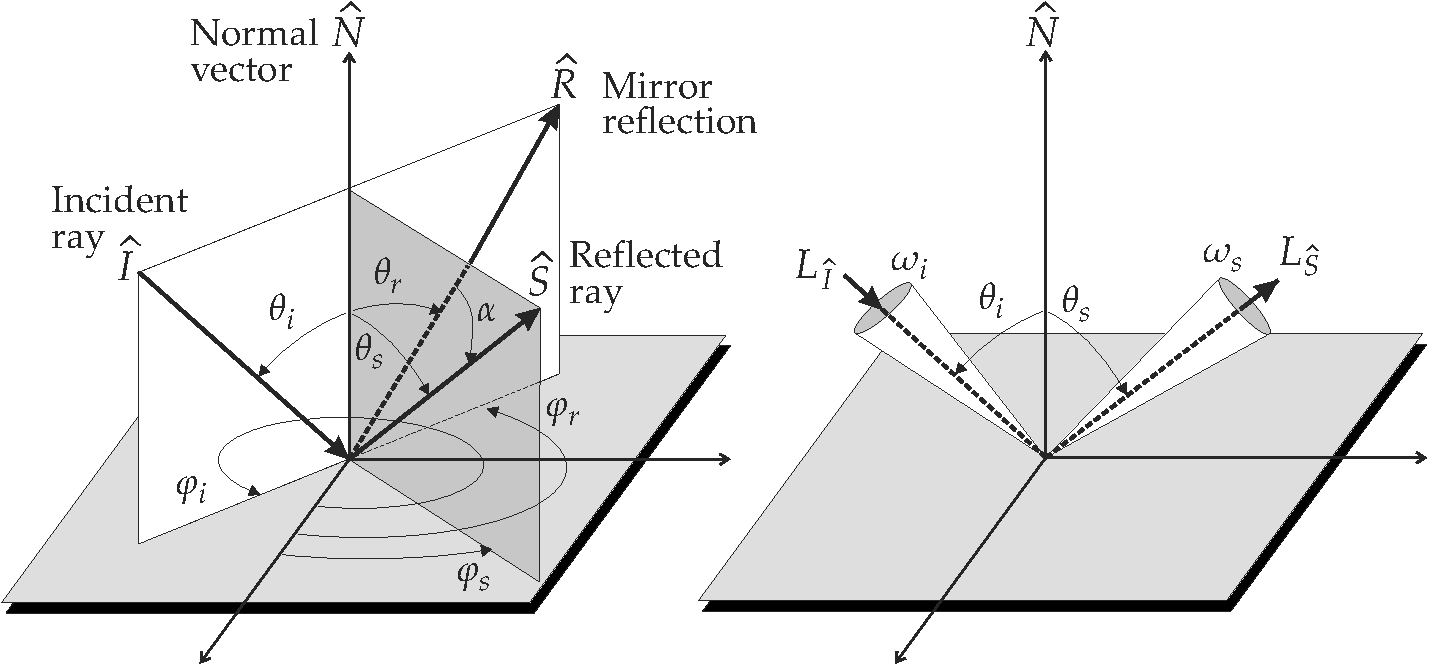
\includegraphics{pic/specref.pdf}}}
\caption{Reflection geometry, here $\theta_i=\theta_{LO}$.\label{fig:specref}}
\end{figure}

\subsection{Specular reflective surfaces\index{laser rangefinder!specular reflective surface|(}}
\label{rfdetectpaint}
\noindent
\index{bidirectional reflection distribution function (BRDF)!specular reflective surface}If the target has a specularly reflecting surface (see Figure~\ref{nonlambert}), the surface BRDF $f_r$ is used to calculate the reflection as a function of angle of incidence and the view direction angle (see Figure~\ref{fig:specref}). Then 
\begin{equation}
E_R = \frac{f_r(\theta_{LO}, \theta_{OR},\varphi_{LO},\varphi_{OR}
) \Phi_L \tau^2_{a} \cos\theta_{LO}\Upsilon}{ R^2 }. %\frac{\Omega_R}{\Omega_L}
\label{lrfi3}
\end{equation}

The relatively simple \index{bidirectional reflection distribution function (BRDF)!Phong model}\index{Phong BRDF model}Phong phenomenological BRDF model that includes diffuse\index{diffuse!reflectance, Phong BRDF} and specular components is
\begin{equation}
f_{r,{\rm Phong}} = \frac{\rho_d}{\pi} + \frac{\rho_s(n+1)\cos^n\alpha}{2\pi\cos\theta_i},
\label{eq:BRDFequationPhong}
\end{equation}
where the angles are defined in Figure~\ref{fig:specref},
\index{diffuse!reflectance!Phong BRDF model}\index{reflectance!diffuse}$\rho_d$ is the diffuse reflection constant,
$n$ determines the angular divergence of the lobe, and \index{specular reflectance}\index{reflectance!specular}$\rho_s$ determines the peak value or `strength' of the lobe. Energy conservation requires that $\rho_s + \rho_d = \rho$, where $\rho=\Phi_r/\Phi_i$ is the total reflected flux divided by the total incident flux. The Phong model is not a  mathematically compliant BRDF because for large $\alpha$ the BRDF value could be negative (i.e., the lobe enters below the surface) --- and if the BRDF value is set to zero for such cases, the law of energy conservation is violated.  The Phong model therefore fails at large $\alpha$ angles and for small $n$. The Phong model also does not comply with the requirement for reciprocality.  There are several variations on the Phong theme that attempt to achieve increased accuracy.  Four typical Phong specular reflection profiles are shown in Figure~\ref{fig:brdfPhongProfiles}.


\begin{figure}[bt]
\centering
\resizebox{\textwidth}{!}{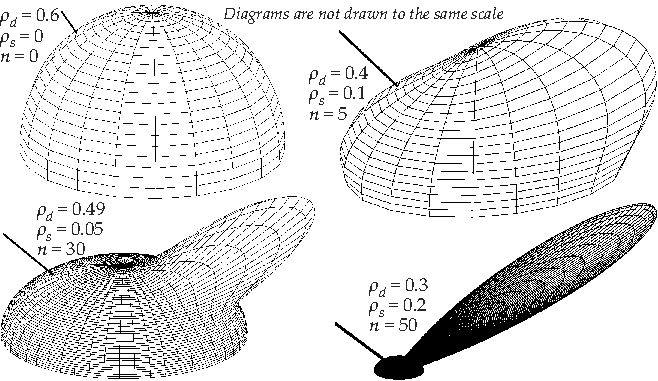
\includegraphics{pic/brdfPhongProfiles.pdf}}
\caption{BRDF calculated by the simple Phong equation. \label{fig:brdfPhongProfiles}}
\end{figure}


Measurements on several paints and natural
surfaces\cite{Bergh2004} indicated Phong model BRDF values as shown in
Table~\ref{brdftab} and Figure~\ref{specref1}. The application of this data toward a laser rangefinder performance calculation is presented in Section~\ref{rfdetectpaint}.

%old \begin{equation}
%BRDF(\theta,\alpha)=
%\frac{\rho_{d_\theta}}{\pi}\cos \theta^\prime+
%\frac{(n+1)\rho_{s_\theta}}{2\pi}\cos^{n_\theta} \alpha
%\end{equation}

\begin{figure}[tb]
\centering
\resizebox{0.8\textwidth}{!}{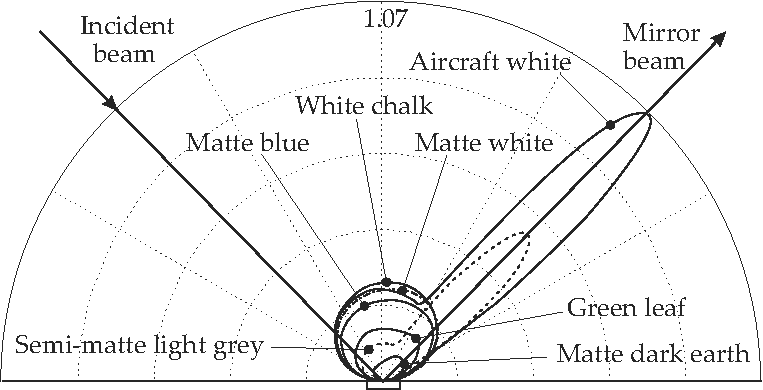
\includegraphics{pic/specref1.pdf}}
\caption{Phong BRDF for paints and natural surfaces in the NIR spectral band.
\label{specref1}}
\end{figure}


\begin{table}[tb]
\centering
\caption{Phong BRDF parameters for paints and natural surfaces in the \index{nearinfrared@near-infrared (NIR)!Phong BRDF parameters}NIR spectral band.\label{brdftab}}
%\vspace{-5mm}
{\small
\begin{tabular}{|l|c|c|c|}
\hline
\textbf{Surface finish} &\multicolumn{3}{c|}{\textbf{0.75--1.4-\si{\micro\metre}{} NIR band}} \\
\cline{2-4}
 & $\bm{ \rho_o}$& $\bm{\rho_s}$ & $\bm{n}$ \\
\hline
Matte dark earth paint & 0.11 & 0.033 & 6\\
Matte blue paint & 0.52 & 0.022 & 8\\
Matte white paint & 0.58 & 0.03 & 6\\
Semi-matte light grey paint & 0.25 & 0.052 & 44\\
Aircraft white paint & 0.6 & 0.05 & 80 \\
%\hline
%Navy light grey & 0.15 & 0.11 & 250\\
%Sea grey & 0.09 & 0.053 & 130\\
\hline
Natural soil & 0.33 & & \\
Sea sand & 0.49 && \\
Green leaf & 0.43 & 0.015 & 15\\
Gypsum / white chalk & 0.77 & 0.044 & 3\\
Steel plate, freshly coated with Zn& 0.05 & 0.39 & 160\\
%Brick & 0.35 & & \\
Concrete & 0.55 & & \\
\hline
\end{tabular}
}
\end{table}


\FloatBarrier


If the surface reflection can be modeled by the Phong equation [\myeqno{eq:BRDFequationPhong}, Figure~\ref{fig:brdfPhongProfiles}], the irradiance at the receiver becomes
\begin{equation}
E_R = 
\left(
\frac{\rho_d}{\pi} + \frac{\rho_s(n+1)\cos^n\alpha}{2\pi\cos\theta_{LO}}
\right)
\left(\frac{
\Phi_L \tau^2_{a} \cos\theta_{LO}\Upsilon}{ R^2 } %\frac{\Omega_R}{\Omega_L}
\right),
\label{lrfi4}
\end{equation}
where the angles $\alpha$ and $\theta_{LO}=\theta_i$ follow from the geometry given in Figure~\ref{fig:specref}. Note that in the case of a laser rangefinder, the transmitter and receiver beams are co-axial, with the result that the $\widehat{I}$ and $\widehat{S}$ vectors align on the same axis, and hence $\theta=\theta^\prime$ and $\alpha=2\theta$.

Using the information in Figure~\ref{specref1}, \myeqno{laserrxn} and the values $\Upsilon = 1$, 
$\Delta f=66$~MHz, $A_d=4.6\times10^{-6}$~m$^2$,
$D^\ast=6\times10^{11}$~cm$\cdot$$\sqrt{\rm Hz}$/W, $A_1=2\times10^{-3}$~m$^2$,
and $\tau_r=0.5$, a sensor noise level of 3~\si{\micro\watt}{} is calculated.
Assume further that a SNR of 5 is required for
operation. The operating range is then determined by solving for $R$ in
\begin{equation}
15\times 10^{-6} = \left(
\frac{\rho_{d_\theta}\cos \theta_{LO}}{\pi}+
\frac{(n+1)\rho_{s_\theta}\cos^n (2\theta_{LO})}{2\pi}
\right)
\left(\frac{
\Phi_L \exp^{-2\gamma R}}{ R^2 }
\right),
\label{lrfi5}
\end{equation}
where the laser power $\Phi_L=4$~MW, and $\gamma=1.5\times10^{-3}$~[1/m].

In this configuration (co-axial receiver and transmitter) strong specular reflection toward the receiver can only occur when the surface normal vector faces the rangefinder, i.e., $\theta_{LO}=0$. By solving the equation for a few of the materials shown in Figure~\ref{specref1}, the detection ranges in Figure~\ref{specref2} were obtained.

\begin{figure}[h]
    \centering
    \resizebox{\textwidth}{!}{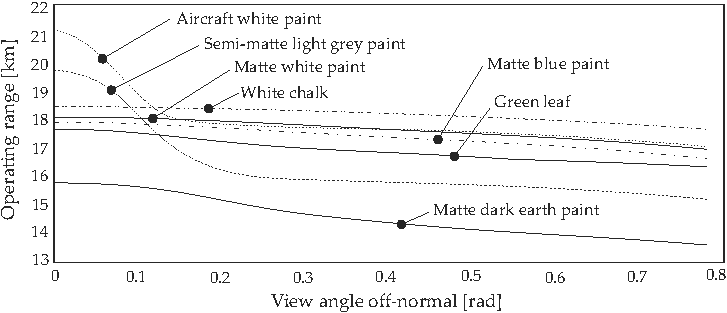
\includegraphics{pic/specref2.pdf}}
    \caption{\label{specref2}Detection range for painted and natural surfaces.}
    \end{figure}

\begin{enumerate}[1.]

\item
In Figure~\ref{specref2}, note the effect of surface properties on range, and in particular, range as a function of off-normal angle.
%
%\item The relatively high similarity in BRDF of the matte white and
%the white paints warrants more investigation. The strong specular
%peak evident in the white is expected, but strangely, the
%diffuse component was no lower than for the matte paint. One would expect
%the `integral under the curve' (which is the total reflected power) to
%be the same in both cases.
%
%Figure~\ref{specref2} shows the expected detection range versus view
%angle for the white in a dotted line. This issue requires more
%investigation.

\item
Except for the white paint anomaly, Figure~\ref{specref2} shows that specular surfaces support longer detection ranges along the mirror reflection vector but lower detection ranges elsewhere. Lambertian surfaces, on the other hand, support a near-constant detection range irrespective of view angle. This is the infrared/optical equivalent of the radar geometric stealth concept. The white paint anomaly requires that this statement be closely investigated.

\item
The sevenfold drop in diffuse reflectance between white chalk and matte dark earth paint, 0.77 to 0.11, resulted in a detection-range ratio of only 1.2. This indicates the relative robustness of the detection process against paint variations. The `compression' in detection range is due to the $1/d^2$ term as well as the severe atmospheric attenuation at longer ranges.

This compression effect will be less severe in a moderate atmosphere.

\item
The fivefold drop between the specular peak and diffuse reflectance for the specular paints only results in a detection range improvement of 1.2 times. The argument is the same as  above.

This compression effect will be less severe in a moderate atmosphere.


\item 
From these results, it would appear that extraordinary attempts to reduce the laser signature by utilizing specular properties or low reflectance values are probably not worth the effort.


%\item
%The quality of the data and reasoning presented here is not very high.
%A more detailed study with practical measurements may be necessary to
%reach conclusive recommendations.

\end{enumerate}

\index{laser rangefinder!specular reflective surface|)}

\index{case study!laser rangefinder range equation|)}\index{laser rangefinder!range equation case study|)} 

